\documentclass[a4paper,11pt]{article}
\usepackage[utf8]{inputenc}
\usepackage[portuguese]{babel}
%\usepackage[backend=bibtex]{biblatex}
%\addbibresource{bibliografia.bib}
\usepackage{enumerate}
\usepackage{multirow}
\usepackage{array}
\usepackage{graphicx}
\usepackage{subfigure}
\usepackage{amssymb, amsmath, amsbsy} 
\usepackage{upgreek} 
\usepackage{cancel} 
\usepackage{mathdots} 
\usepackage{mathrsfs} 
\usepackage{stackrel} 

\usepackage{fancyhdr}
\pagestyle{fancy}
\fancyhf{}
\chead{\begin{picture}(0,0) \put(-210,0){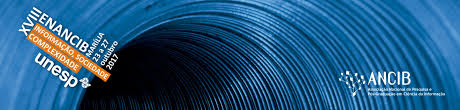
\includegraphics[width=1.2\textwidth]{./enacib}} \end{picture}}
\cfoot{}
\rfoot{\thepage}
\usepackage[table,xcdraw]{xcolor}
\usepackage{hyperref}


\begin{document}
\title{AS FORMAS DA INFORMAÇÃO: UM OLHAR AOS CONCEITOS DE INFORMAÇÃO E FLUXO DE INFORMAÇÃO}
\author{Paloma Marín Arraiza$^{1}$, Jorge Manuel Bolaños Carmona$^{2}$, \\
Silvana Aparecida Borsetti Gregorio Vidotti $^{3}$\\ \\
\small{$^{1-3}$Universidade Estadual Paulista (UNESP), $^{2}$Universidad de Granada (UGR).}\\
}
\date{}
\maketitle
\begin{abstract}
$\href{https://github.com/pmarrai/proyecto_final}{URL \ del \ repositorio}$.\\

Na Ciência da Informação convivem diferentes abordagens ao conceito de informação. Para fornecer uma maior compreensão do fenômeno da informação realiza-se um estudo das diferentes definições específicas da informação e dos fluxos informacionais no contexto da Ciência da Informação, sem esquecer a influência e relevância de outras áreas do conhecimento no estabelecimento destas definições e abordagens. Este estudo baseia-se nos resultados e na releitura de uma pesquisa de mestrado defendida no ano 2014. Utilizou-se uma metodologia bibliográfica e analítica para a investigação teórica dos temas abordados, mantendo uma abordagem qualitativa para o estudo dos conceitos de informação e fluxos informacionais. \\

$\bf{Palavras-chave}$: Teoria Matemática da Informação; conceitos da informação; fluxo de
informação, formas da informação.
\end{abstract}

\begin{table}[hp]
\begin{center}
\begin{tabular}{| m{13cm} |}
\hline
{\color[HTML]{FE0000} Este artículo está compuesto de fragmentos de un trabajo presentado en 2017 en el XVIII Encontro Nacional de Pesquisa em Ciência da Informação en Brasil.
 Por lo tanto, no tiene sentido de principio a fin y hay imágenes (p.ej. \ref{fig:foto1}) que no están en el texto original, pero se han introducido aquí para cumplir los requisitos del curso.
 El texto completo puede leerse en \href{http://enancib.marilia.unesp.br/index.php/xviiienancib/ENANCIB/paper/view/167}{la página del evento}.}\\ \hline
\end{tabular}
\end{center}
\end{table}

\cleardoublepage
\section{Introdução}

A imprensa, o rádio e a atual Internet têm envolvido mudanças importantes na
maneira em que a humanidade tem interagido com a informação e a geração de fluxos de
informação. Porém, provavelmente seja no século XXI quando tenhamos vivenciado um maior
impacto no crescimento da informação. \\

Embora atualmente sejamos mais conscientes do excesso de informação (\textit{information
overload}) e da necessidade de desenvolver melhores tecnologias para o armazenamento e a
recuperação, diversos pesquisadores datam o maior boom informacional no ano 1945, ao
acabar a Segunda Guerra Mundial. Nesse ano, pesquisas e documentos mantidos até o
momento fora no fluxo normal de informação foram liberados para ser colocados à disposição
do conhecimento coletivo \cite{barr1}. \\

A partir de 1945, surgem diferente modelos e teoria sobre a informação e a
transferência dela. O mais conhecido inicia-se nos anos 1948 e 1949 quando Shannon e
Weaver propõem um modelo de transferência da informação composto por uma fonte
geradora, um codificador, uma mensagem, um canal, um decodificador e um receptor. Ao
começo, este modelo era puramente técnico e aplicado à transmissão de sinais: de aí surgiu a
abordagem matemática-probabilística da informação. Porém, o aumento do conteúdo
informacional que estava acontecendo na época e as necessidades de adopção de um modelo
de comunicação humana fizeram que o modelo de Shannon e Weaver fosse adoptado para
analisar situações comunicativas além da probabilidade de transmissão de um sinal. Isto fez
com que conceitos expostos neste modelo permeassem em outras abordagens como a
cognitiva \cite{belk}.\\

\section{Percurso metodológico}

Para este trabalho utilizou-se uma metodologia bibliográfica e analítica para a
investigação teórica dos temas abordados, mantendo uma abordagem qualitativa para o
estudo dos conceitos de informação e fluxos informacionais.\\
Primeiramente, realizou-se uma análise bibliográfica dos temas tratados com o fim de
obter conhecimentos teóricos sobre o conceito de informação e os fluxos informacionais. Na
análise bibliográfica, pretendeu-se esclarecer as diferentes abordagens do conceito de
informação existentes na literatura, bem como as implicações teóricas delas que possam 
contribuir ao entendimento dos fluxos informacionais e as mudanças que têm experimentado.
Os critérios para a eleição do material bibliográfico foram assuntos relativos ao tema em
artigos científicos escritos em espanhol, inglês e português entre os anos 1948 y 2014 achadas
nas bases Google Scholar, SciELO e Dialnet (ver \ref{tabla:uno}).\\

\begin{table}[h]
\begin{center}
\begin{tabular}{| l | c | c | c |}
\hline
\textbf{Língua (palavra-chave)}               & \textbf{Google Scholar} & \multicolumn{1}{l|}{\textbf{SciELO}} & \multicolumn{1}{l|}{{\color[HTML]{000000} \textbf{Dialnet}}} \\ 
\hline \hline
Espanhol (concepto de información)            & 17                      & 6                                    & 71                                                           \\ \hline
Inglês (concept of information)               & 30                      & 13                                   & -                                                            \\ \hline
Português (conceito da informação)            & 29                      & 73                                   & -                                                            \\ \hline
Espanhol (Teoría Matemática de la infomación) & 29                      & -                                    & 5                                                            \\ \hline
Inglês (Mathematical Information Theory)      & 24                      & -                                    & 1                                                            \\ \hline
Português (Teoria Matemática da Informação)   & 20                      & -                                    & -                                                         \\ \hline
\end{tabular}
\caption{Número de artigos recuperados por base de dados, língua e palavra-chave. Fonte: Elaboração dos autores.}
\label{tabla:uno}
\end{center}
\end{table}

Dos documentos recuperados eliminaram-se aqueles repetidos em diferentes bases,
bem como aqueles que não abordavam os conceitos desde a Ciência da Informação e sim
desde outras áreas como a Computação, Física Quântica, Administração, Negócios, Educação
e Jornalismo. Se bem, a presença dos conceitos nestas áreas permite entender a abrangência
do termo. \\
Finalmente, para a pesquisa de mestrado, foram analisados 59 documentos, sendo
alguns considerados repetitivos e não citados na dissertação final. Os documentos foram
completados também com documentos do acervo bibliotecário da instituição, chegando aos
67 documentos consultados.\\

\begin{figure}[hp]
\centering
\subfigure[Palavras chave]{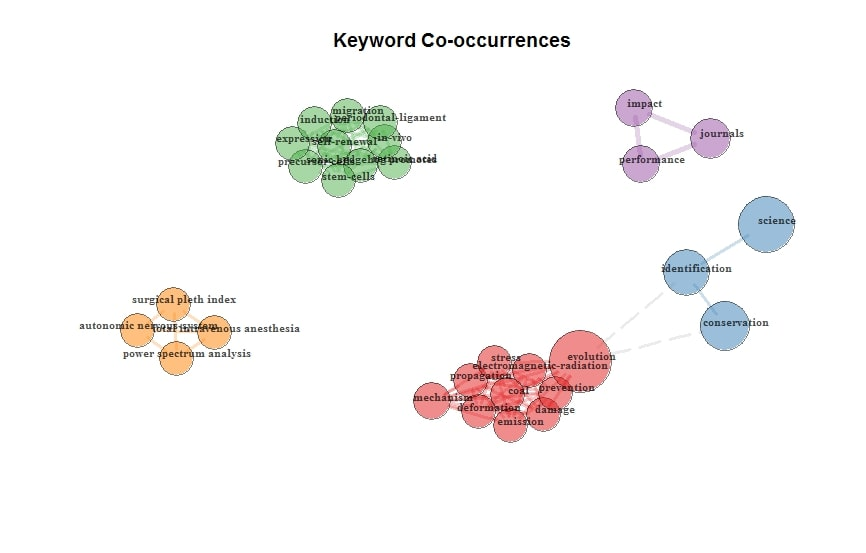
\includegraphics [width=\textwidth]{kyword}}
\subfigure [Países]{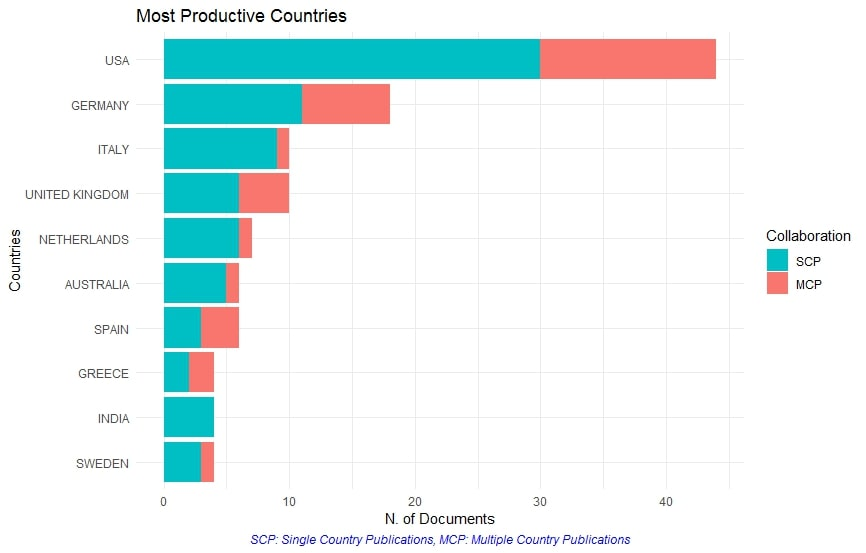
\includegraphics [width=\textwidth]{productive}}
\caption{Análise de palavras chave e produtividade}
\label{fig:img1}
\end{figure}

\section{A multiplicidade da informação}

Ao longo da literatura, observam-se duas abordagens majoritárias ao conceito de informação: informação como algo físico, objetivo e informação como algo subjetivo \cite{fer}. 
A informação é considerada tanto “conteúdo objetivo”, medível, transportável e armazenável quanto o resultado da interação entre dados e o estado do conhecimento de um sujeito \cite{ara}.
Porém, também há abordagens que indicam quatro usos básicos do termo: informação como entidade física; informação como processo mental de se informar; informação como construção social (e o compartilhamento dela segundo o sistema social) e informação como probabilidade de que uma determinada mensagem seja enviada.

\subsection{A Abordagem Matemático-Probabilística da Informação}

A primeira metade do século XX caracterizou-se pelo desenvolvimento das
comunicações eletrônicas. Em 1924, Nyquist publicou o artigo Certain Factors affecting the
Telegraph Speed no que discutia a velocidade de transmissão da inteligência. Em 1928, Hartley
propus a primeira variante da medição da informação aplicando a Teoria Matemática de
probabilidades \cite{sok} .
Pouco depois nasce a era dos
computadores graças a Shestakov (em 1935), Shannon (em 1938), Turing (em 1936) e von
Newmann (em 1944) \cite{berr}.
Na termodinâmica, a entropia indica o grau de desordem de um sistema. Shannon
utiliza a probabilidade de que um sucesso ou mensagem aconteça dentro do conjunto dos
sucessos possíveis sem que estes devam ser equiprováveis. Cada sucessor possui uma
probabilidade, $p_{i}$. Assim a entropia é definida como: 

\begin{equation}
H_{i} = - \sum_{i=1}^{n} p_{i} \log(p_{i})
\label{eq:equ1}
\end{equation}

$H_{i}$ é a entropia global da mensagem, baseada na definição de Boltzmann para a entropia de um processo mecânico-estatístico. O valor máximo da entropia (H = I) aconteceria se todos os sucessos tiverem a mesma probabilidade ($p = \frac{1}{n}$).

\subsection{A Abordagem Cognitiva da Informação}


Os conceitos matemáticos não perdem importância. De fato, a quantificação, ou até matematização, das estruturas do conhecimento está presente também nas abordagens cognitivas. No ano 1974, Bertram Brookes propus a “equação fundamental da Ciência da Informação”:

\begin{equation}
K[S] + \Delta I = K[S + \Delta S]
\label{eq:equ2}
\end{equation}

Onde a estrutura do conhecimento  $(K[S])$ é modificada pela informação $(\Delta I)$ e resulta a forma $K[S + \Delta S]$, sendo $\Delta S$ efeito da modificação. Nesta expressão, tanto a informação como o conhecimento teriam a mesma dimensão e se condicionariam entre si. \\
\begin{figure}[h]
\centering
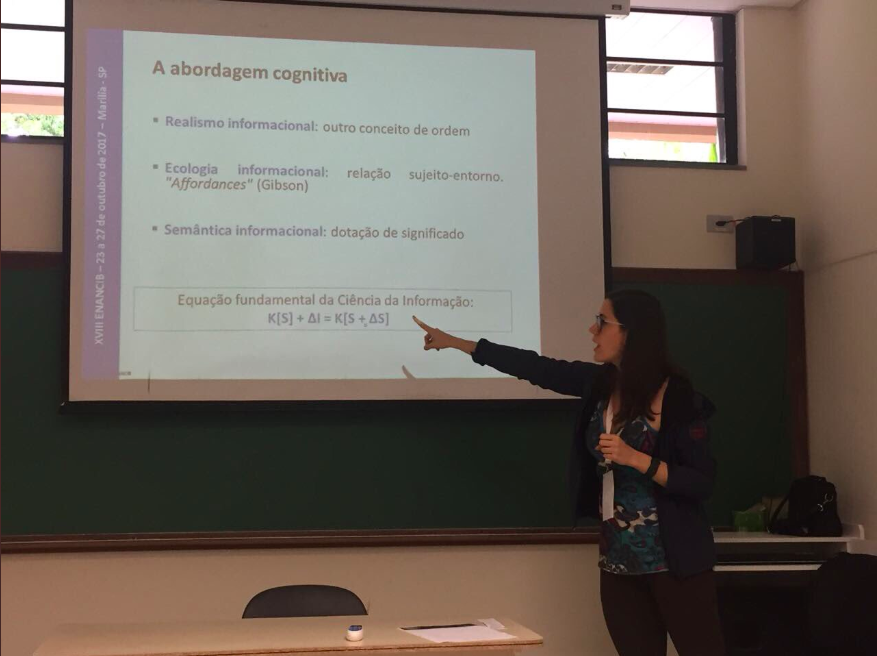
\includegraphics[width=0.7\textwidth]{./foto1}
\caption{Foto tomada no dia da apresentação} \label{fig:foto1}
\end{figure}\\

Na semântica informacional, os estudos tentam explicar a natureza da informação que é outorgada pelo significado. Porém, os processos informacionais analisados guardam uma estreita relação com a Teoria Matemática da Informação. A Teoria Matemática da Informação e a Teoria Semântica da Informação são formalmente análogas \cite{bar}. Conceitos como ruído do canal, eficiência do código e redundância do código da primeira correspondem com ruído semântico, eficiência e redundância do marco conceptual de trabalho da segunda. Neste sentido, \cite{dre} propõe a definição nuclear de informação para explicar o conteúdo informacional de um sinal:
\begin{center}
    \begin{minipage}{0.7\linewidth}
        \vspace{5pt}
        {\small 
          (...) um sinal carrega informação (nuclear) sobre o que ocorre em uma fonte (expressando o seu conteúdo) se ele for capaz de reproduzir factualmente as relações que se estabelecem na fonte, tornando-as acessíveis para qualquer observador que se encontre em condições de recebê-las \cite[p. 9]{gon}.
        }
        \vspace{5pt}
    \end{minipage}
\end{center}
Ainda, “(...) o conteúdo informacional pode ser explicado a través de sua digitalização” \cite[p. 9]{gon}. Segundo estes três autores, a hipótese central dretskeana centra-se na digitalização: digitalizar um sinal garante a especificidade da informação percebida. A percepção da informação é realizada a través de um filtro de informação analógica, entendida como a possibilidade de que um sinal aporte informação adicional sobre a mensagem que transmite.

\section{Os fluxos de informação}

\subsection{Os Fluxos de Informação nas Culturas Auditiva, Textual e Eletrônica}
Os roles de emissor e receptor podem não ser fixos durante o processo de transmissão, e consequente fluxo, de informação. A informação entra dentro de um fluxo helicoidal que faz com que se renove continuamente. Neste sentido, Barreto (1998), propõe um esquema do ciclo da informação:
\begin{equation}
\underbrace{(info_{1})}_{primeira \ parte \ do \ ciclo} \rightarrow conhecimento \rightarrow desenvolvimento \rightarrow \overbrace{(info_{2})}^{resultado}
\label{eq:equ3}
\end{equation}
\\
A passagem da cultura escrita à eletrônica envolve também a passagem do mundo
analógico ao digital. Castro \footnote{O exposto pela autora tem sido ampliado com os comentários de outros autores e próprios.} identifica alguns fatores que determinam as diferencias
entre ambos.
\begin{enumerate}
\item $\textit{O trânsito à sociedade do conhecimento}$. O rol do receptor varia, já não é mais um
receptor passivo de informações, senão que se envolve na geração de novo.
\item $\textit{A redução da intermediação na informação circulante}$. Cada sujeito é emissor de
informação, motivo pelo qual não são tão necessárias as grandes empresas de
comunicação. Estamos ante uma situação de multiplicidades nas fontes.
\end{enumerate}
\section {Considerações finais}
Este trabalho teve como objetivo fornecer uma maior compreensão do fenômeno da
informação mediante o estudo das diferentes definições específicas do conceito de
informação e dos fluxos informacionais dentro do contexto da CI. \\
Para isso, considerou-se acertado o posicionamento de \cite{ara10} segundo o pesquisado por \cite{capu}:
considerar quatro vertentes da informação. Das quatro vertentes foram abordadas três: a
matemático-estatística, a visão cognitiva e o conceito de Buckland (informação como coisa). \\

É importante destacar que em cada vertente são desenvolvidos conceitos particulares da
informação. Estes são, às vezes, semelhantes entre eles, sobrepostos ou discordantes
. O estudo do fenômeno da informação abrange, também, os canais e o fluxos
de informação integrados nos processos de comunicação. A análise das vertentes e os fluxos
resultou em um novo olhar ao conceito de informação: a forma estrutural, a forma dinâmica
e a forma comunicada.

\cleardoublepage
\bibliography{bibliografia}
\bibliographystyle{plain}
\end{document}